\documentclass[12pt,letterpaper]{article}
\usepackage{graphicx,textcomp}
\usepackage{natbib}
\usepackage{setspace}
\usepackage{fullpage}
\usepackage{color}
\usepackage[reqno]{amsmath}
\usepackage{amsthm}
\usepackage{fancyvrb}
\usepackage{amssymb,enumerate}
\usepackage[all]{xy}
\usepackage{endnotes}
\usepackage{lscape}
\newtheorem{com}{Comment}
\usepackage{float}
\usepackage{hyperref}
\newtheorem{lem} {Lemma}
\newtheorem{prop}{Proposition}
\newtheorem{thm}{Theorem}
\newtheorem{defn}{Definition}
\newtheorem{cor}{Corollary}
\newtheorem{obs}{Observation}
\usepackage[compact]{titlesec}
\usepackage{dcolumn}
\usepackage{tikz}
\usetikzlibrary{arrows}
\usepackage{multirow}
\usepackage{xcolor}
\newcolumntype{.}{D{.}{.}{-1}}
\newcolumntype{d}[1]{D{.}{.}{#1}}
\definecolor{light-gray}{gray}{0.65}
\usepackage{url}
\usepackage{listings}
\usepackage{color}

\usepackage{verbatim}
%\usepackage[utf8]{inputenc}
\usepackage[T1]{fontenc}

\definecolor{codegreen}{rgb}{0,0.6,0}
\definecolor{codegray}{rgb}{0.5,0.5,0.5}
\definecolor{codepurple}{rgb}{0.58,0,0.82}
\definecolor{backcolour}{rgb}{0.95,0.95,0.92}

\lstdefinestyle{mystyle}{
	backgroundcolor=\color{backcolour},   
	commentstyle=\color{codegreen},
	keywordstyle=\color{magenta},
	numberstyle=\tiny\color{codegray},
	stringstyle=\color{codepurple},
	basicstyle=\footnotesize,
	breakatwhitespace=false,         
	breaklines=true,                 
	captionpos=b,                    
	keepspaces=true,                 
	numbers=left,                    
	numbersep=5pt,                  
	showspaces=false,                
	showstringspaces=false,
	showtabs=false,                  
	tabsize=2
}
\lstset{style=mystyle}
\newcommand{\Sref}[1]{Section~\ref{#1}}
\newtheorem{hyp}{Hypothesis}

\title{Problem Set 2}
\date{Due: February 19, 2023}
\author{Applied Stats II}


\begin{document}
	\maketitle
	\section*{Instructions}
	\begin{itemize}
%		\item Please show your work! You may lose points by simply writing in the answer. If the problem requires you to execute commands in \texttt{R}, please include the code you used to get your answers. Please also include the \texttt{.R} file that contains your code. If you are not sure if work needs to be shown for a particular problem, please ask.
%		\item Your homework should be submitted electronically on GitHub in \texttt{.pdf} form.
		\item This problem set is due before 23:59 on Sunday February 19, 2023. No late assignments will be accepted.
	%	\item Total available points for this homework is 80.
	\end{itemize}

	
	%	\vspace{.25cm}
	
	Code in \texttt{PS2\_ImeldaFinn.R}

%\section*{Question 1} %(20 points)}
\vspace{.25cm}
\noindent We're interested in what types of international environmental agreements or policies people support (\href{https://www.pnas.org/content/110/34/13763}{Bechtel and Scheve 2013)}. So, we asked 8,500 individuals whether they support a given policy, and for each participant, we vary the (1) number of countries that participate in the international agreement and (2) sanctions for not following the agreement. \\

%\noindent Load in the data labeled \texttt{climateSupport.csv} on GitHub, which contains an .

\begin{itemize}
  \item observational study of 8,500 observations
	\item Response variable: 
	\begin{itemize}
		\item \texttt{choice}: 1 if the individual agreed with the policy; 0 if the individual did not support the policy
	\end{itemize}
	\item Explanatory variables: 
	\begin{itemize}
		\item
		\texttt{countries}: Number of participating countries [20 of 192; 80 of 192; 160 of 192]
		\item
		\texttt{sanctions}: Sanctions for missing emission reduction targets [None, 5\%, 15\%, and 20\% of the monthly household costs given 2\% GDP growth]
		
	\end{itemize}
	
\end{itemize}

  Read in the data and modified \texttt{choice} variable:
  
    \begin{lstlisting}[language=R]
    load(url("https://github.com/ASDS-TCD/StatsII_Spring2023/blob/main/datasets/climateSupport.RData?raw=true"))
    # choice = 1,2
    # countries = 1, 2, 3
    # sanctions = 1, 2, 3, 4

    # get a version of the dataset with the response variable coded as 
    # True = supported
    # False = not supported
    cs <- climateSupport
    cs$choice <- as.logical(as.numeric(cs$choice)-1) 
    
    summary(cs)
    ...
    
       choice             countries    sanctions  
    Mode :logical   20 of 192 :2865   None:2119  
    FALSE:4264      80 of 192 :2795   5%  :2133  
    TRUE :4236      160 of 192:2840   15% :2111  
                                      20% :2137  
  \end{lstlisting}

%\noindent Please answer the following questions:

\begin{enumerate}
	\item
	Remember, we are interested in predicting the likelihood of an individual supporting a policy based on the number of countries participating and the possible sanctions for non-compliance.
	\begin{enumerate}
		\item [] Fit an additive model. 

      \lstinputlisting[language=R, firstline=105, lastline=105]{PS2_ImeldaFinn.R}
		
		\item Summary output, 

    \begin{lstlisting}[language=R]

      Call:
      glm(formula = choice ~ ., family = binomial(link = "logit"), 
          data = cs)

      Deviance Residuals: 
          Min       1Q   Median       3Q      Max  
      -1.4259  -1.1480  -0.9444   1.1505   1.4298  

      Coefficients:
                   Estimate Std. Error z value Pr(>|z|)    
      (Intercept) -0.005665   0.021971  -0.258 0.796517    
      countries.L  0.458452   0.038101  12.033  < 2e-16 ***
      countries.Q -0.009950   0.038056  -0.261 0.793741    
      sanctions.L -0.276332   0.043925  -6.291 3.15e-10 ***
      sanctions.Q -0.181086   0.043963  -4.119 3.80e-05 ***
      sanctions.C  0.150207   0.043992   3.414 0.000639 ***
      ---
      Signif. codes:  0 '***' 0.001 '**' 0.01 '*' 0.05 '.' 0.1 ' ' 1

      (Dispersion parameter for binomial family taken to be 1)

          Null deviance: 11783  on 8499  degrees of freedom
      Residual deviance: 11568  on 8494  degrees of freedom
      AIC: 11580

      Number of Fisher Scoring iterations: 4
    \end{lstlisting}
    \begin{figure}[!htbp]
	    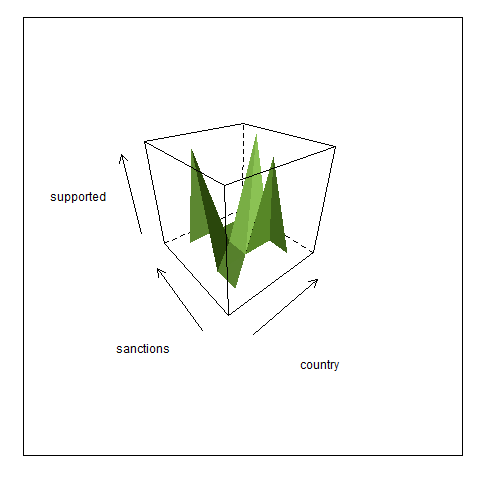
\includegraphics[width=0.85\textwidth]{graphics/wireframe.png}
	    \caption{plot of additive (glm) model}
	    \label{fig:glm}
	\end{figure}

		\item The global null hypothesis and $p$-value. 
		
		$H_0$: the explanatory variables have no effect on the likelihood of an individual supporting a policy
		
		$H_a$: one or more of the explanatory variables have some effect on the likelihood of an individual supporting a policy

    $\alpha = 0.05$
    
    The data was modelled with no explanatory variables ($choice \tilde~1$). %TODO
    The comparison of the two models is shown in ~\ref{tab:glm:null}
      \lstinputlisting[language=R, firstline=131, lastline=131]{PS2_ImeldaFinn.R}

      A test was run to compare the deviances of the two models.
      
      \lstinputlisting[language=R, firstline=136, lastline=136]{PS2_ImeldaFinn.R}
      The results are shown in ~\ref{tab:anova}.  
      The $\chi^2$ statistic = $11783 - 11568 = 215.15$. The assocated p-value with 5 degrees of freedom is $2.2\times 10^{-16}$.  
      
      As the p-value is below $\alpha$ we reject the null hypothesis.  The evidence does not support the assumption that none of the explanatory variables have any effect on our response variable \texttt{choice}.  We expect that one or more of our explanatory variables will have a statistically significant effect on the probability of a policy being supported.

			
% Table created by stargazer v.5.2.3 by Marek Hlavac, Social Policy Institute. E-mail: marek.hlavac at gmail.com
% Date and time: Fri, Feb 17, 2023 - 23:19:51
\begin{table}[!htbp] \centering 
  \caption{} 
  \label{tab:glm:null} 
\begin{tabular}{@{\extracolsep{5pt}}lcc} 
\\[-1.8ex]\hline 
\hline \\[-1.8ex] 
 & \multicolumn{2}{c}{\textit{Dependent variable:}} \\ 
\cline{2-3} 
\\[-1.8ex] & \multicolumn{2}{c}{choice} \\ 
\\[-1.8ex] & \multicolumn{2}{c}{\textit{logistic}} \\ 
\\[-1.8ex] & (1) & (2)\\ 
\hline \\[-1.8ex] 
 countries:  80 of 192 & 0.458$^{***}$ &  \\ 
  & (0.038) &  \\ 
  & & \\ 
 countries:  160 of 192 & $-$0.010 &  \\ 
  & (0.038) &  \\ 
  & & \\ 
 sanctions: 5\% & $-$0.276$^{***}$ &  \\ 
  & (0.044) &  \\ 
  & & \\ 
 sanctions: 5\% & $-$0.181$^{***}$ &  \\ 
  & (0.044) &  \\ 
  & & \\ 
 sanctions: 5\% & 0.150$^{***}$ &  \\ 
  & (0.044) &  \\ 
  & & \\ 
 Constant & $-$0.006 & $-$0.007 \\ 
  & (0.022) & (0.022) \\ 
  & & \\ 
\hline \\[-1.8ex] 
Observations & 8,500 & 8,500 \\ 
Log Likelihood & $-$5,784.130 & $-$5,891.705 \\ 
Akaike Inf. Crit. & 11,580.260 & 11,785.410 \\ 
\hline 
\hline \\[-1.8ex] 
\textit{Note:}  & \multicolumn{2}{r}{$^{*}$p$<$0.1; $^{**}$p$<$0.05; $^{***}$p$<$0.01} \\ 
\end{tabular} 
\end{table}  

% Table created by stargazer v.5.2.3 by Marek Hlavac, Social Policy Institute. E-mail: marek.hlavac at gmail.com
% Date and time: Fri, Feb 17, 2023 - 23:19:55
\begin{table}[!htbp] \centering 
  \caption{} 
  \label{tab:anova} 
\begin{tabular}{@{\extracolsep{5pt}}lccccc} 
\\[-1.8ex]\hline 
\hline \\[-1.8ex] 
Statistic & \multicolumn{1}{c}{N} & \multicolumn{1}{c}{Mean} & \multicolumn{1}{c}{St. Dev.} & \multicolumn{1}{c}{Min} & \multicolumn{1}{c}{Max} \\ 
\hline \\[-1.8ex] 
Resid. Df & 2 & 8,496.500 & 3.536 & 8,494 & 8,499 \\ 
Resid. Dev & 2 & 11,675.830 & 152.134 & 11,568.260 & 11,783.410 \\ 
Df & 1 & 5.000 &  & 5 & 5 \\ 
Deviance & 1 & 215.150 &  & 215.150 & 215.150 \\ 
Pr(\textgreater Chi) & 1 & 0.000 &  & 0 & 0 \\ 
\hline \\[-1.8ex] 
\end{tabular} 
\end{table}  


		\item  Please describe the results and provide a conclusion.
		
		When 20 out of 192 countries are included and there are no sanctions (base case), then the expected odds of a participant agreeing with a policy are $e^{-0.005665} = 0.994351$ 
		
		A one unit increase in $X_k$ increases the odds of supporting a policy by a multiplicative factor of $e^{\beta_k}$

    When 20 out of 192 countries are included and there are sanctions of 5\%, the logodds change by $e^{-0.276332} = 0.758561$ compared to the base
    
    $logit(p) = -0.005665 + -0.276332 $

    When 80 out of 192 countries are included and there are no sanctions, the logodds change by $e^{-0.458453} = 0.632261$ compared to the base
    
    $logit(p) = -0.005665  -0.458453 $

    When 80 out of 192 countries are included and there are sanctions of 5\%, then:
  
    $logit(p) = -0.005665 + -0.276332  -0.458453 = $%exp(-0.005665) *exp(-0.276332) *exp(-0.458453)$
    
    $e^{logit(p)} = 0.4768993$

    ie the odds reduce by 48.0\%.
    
    
    The predicted probabilities, and confidence intervals, are in Table~\ref{tab:pred}
      
%      The $e^{\beta_k}$s are all non-zero and the $5\%$ Confidence Intervals do not include 0.(Table~\ref{tab:CIs}).
      
      The estimates for $\beta_k$ are all significant at $p=0.01$ except for  `countries: 160 of 192' (\texttt{countries.Q}), 
      ie there is a predicted -0.1 change in $logit$ going from 80 to 160 countries, but it is not statistically significant.
      
	    
% Table created by stargazer v.5.2.3 by Marek Hlavac, Social Policy Institute. E-mail: marek.hlavac at gmail.com
% Date and time: Sun, Feb 19, 2023 - 22:30:04
\begin{table}[!htbp] \centering 
  \caption{} 
  \label{tab:pred} 
\begin{tabular}{@{\extracolsep{5pt}} ccccccccc} 
\\[-1.8ex]\hline 
\hline \\[-1.8ex] 
 & countries & sanctions & fit & se.fit & residual.scale & UL & LL & PredictedProb \\ 
\hline \\[-1.8ex] 
6 & 20 of 192 & None & $0.4323$ & $0.0132$ & $1$ & $0.6125$ & $0.6002$ & $0.6064$ \\ 
9 & 20 of 192 & 5\% & $0.4798$ & $0.0133$ & $1$ & $0.6238$ & $0.6115$ & $0.6177$ \\ 
3 & 20 of 192 & 15\% & $0.3999$ & $0.0130$ & $1$ & $0.6048$ & $0.5925$ & $0.5987$ \\ 
12 & 20 of 192 & 20\% & $0.3598$ & $0.0125$ & $1$ & $0.5949$ & $0.5830$ & $0.5890$ \\ 
4 & 80 of 192 & None & $0.5159$ & $0.0134$ & $1$ & $0.6323$ & $0.6200$ & $0.6262$ \\ 
7 & 80 of 192 & 5\% & $0.5635$ & $0.0135$ & $1$ & $0.6434$ & $0.6311$ & $0.6373$ \\ 
1 & 80 of 192 & 15\% & $0.4826$ & $0.0134$ & $1$ & $0.6245$ & $0.6122$ & $0.6184$ \\ 
10 & 80 of 192 & 20\% & $0.4403$ & $0.0131$ & $1$ & $0.6144$ & $0.6022$ & $0.6083$ \\ 
5 & 160 of 192 & None & $0.5928$ & $0.0131$ & $1$ & $0.6499$ & $0.6381$ & $0.6440$ \\ 
8 & 160 of 192 & 5\% & $0.6382$ & $0.0124$ & $1$ & $0.6598$ & $0.6488$ & $0.6543$ \\ 
2 & 160 of 192 & 15\% & $0.5603$ & $0.0132$ & $1$ & $0.6425$ & $0.6305$ & $0.6365$ \\ 
11 & 160 of 192 & 20\% & $0.5180$ & $0.0135$ & $1$ & $0.6329$ & $0.6205$ & $0.6267$ \\ 
\hline \\[-1.8ex] 
\end{tabular} 
\end{table}  

      \begin{figure}[!htbp]
  	    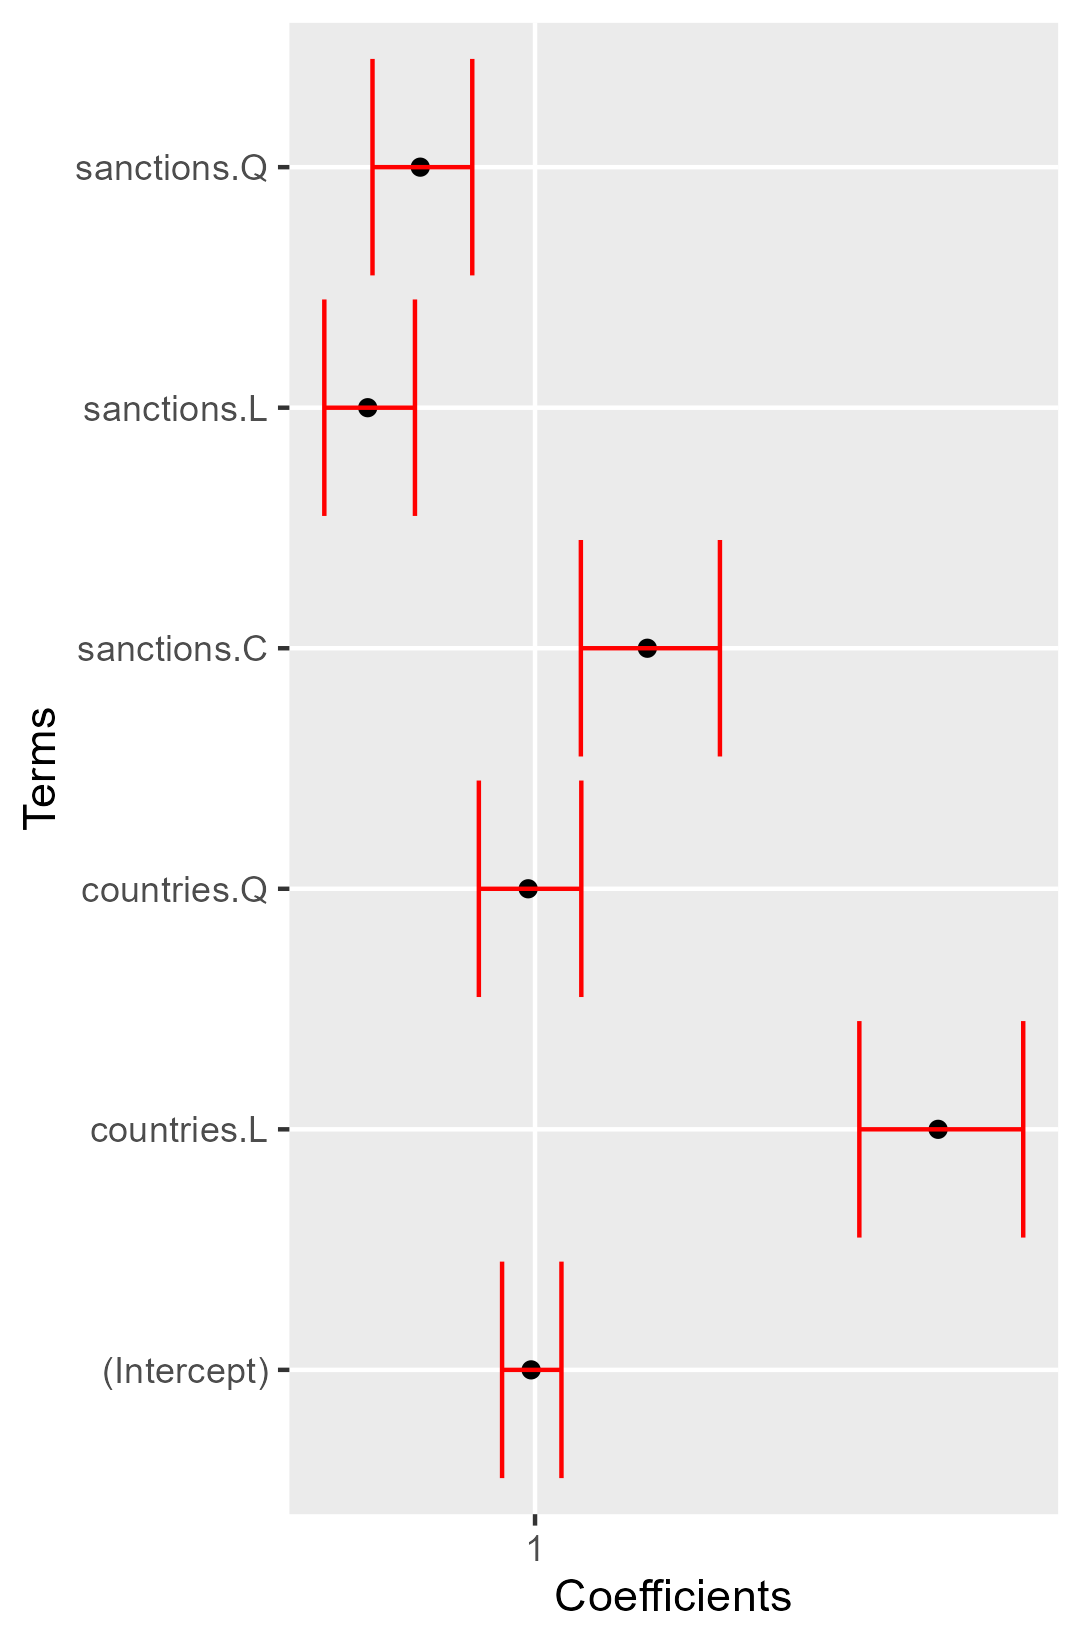
\includegraphics[width=0.8\textwidth]{graphics/coefficients.png}
  	    \caption{coefficients of additive model}
  	    \label{fig:coefs}
	    \end{figure}

		It took 4 iterations to find the maximum likelihood estimates.
		
		The log likelihood is -5,784.130
	\end{enumerate}


	\item
	If any of the explanatory variables are significant in this model, then:
	\begin{enumerate}
		\item
		For the policy in which nearly all countries participate [160 of 192], how does increasing sanctions from 5\% to 15\% change the odds that an individual will support the policy? (Interpretation of a coefficient)
%		\item
%		For the policy in which very few countries participate [20 of 192], how does increasing sanctions from 5\% to 15\% change the odds that an individual will support the policy? (Interpretation of a coefficient)
		\item
		What is the estimated probability that an individual will support a policy if there are 80 of 192 countries participating with no sanctions? 
		\item
		%Would the answers to 2a and 2b potentially change if we included the interaction term in this model? Why? 
		
		Including an interaction term would potentially change the results in 2a and 2b.  The values for the coefficients would potentially be different (eg $beta_{k}$) and we would have to include the constituent coefficient values in calculating the value of the logit.
		
		\begin{itemize}
		%Perform a test to see ifincluding an interaction is appropriate.

			\item A model was run on the data, with an interaction between \texttt{countries} and \texttt{sanctions}, and an ANOVA/$\chi_2$ test was run.  The results are shown in Tables ~\ref{tab:int} and ~\ref{tab:anova:int}.
			
			The test statistic of 6.2928, with 6 degrees of freedom, lead to a p-value of 0.3912.  Therefore we cannot reject the null hypothesis that the two models are the same, ie we do not conclude that an interaction term is appropriate.
			
%286
      \lstinputlisting[language=R, firstline=278, lastline=281]{PS2_ImeldaFinn.R}

      \begin{lstlisting}[language=R]
      int_mod <- glm(choice ~countries + sanctions + countries * sanctions,
               family = binomial(link="logit"), data = cs)

      anova_int <- anova(mod, int_mod, test= "LRT")
      \end{lstlisting}

		  
% Table created by stargazer v.5.2.3 by Marek Hlavac, Social Policy Institute. E-mail: marek.hlavac at gmail.com
% Date and time: Fri, Feb 17, 2023 - 23:50:59
\begin{table}[!htbp] \centering 
  \caption{} 
  \label{tab:int} 
\begin{tabular}{@{\extracolsep{5pt}}lcc} 
\\[-1.8ex]\hline 
\hline \\[-1.8ex] 
 & \multicolumn{2}{c}{\textit{Dependent variable:}} \\ 
\cline{2-3} 
\\[-1.8ex] & \multicolumn{2}{c}{choice} \\ 
\\[-1.8ex] & \multicolumn{2}{c}{\textit{logistic}} \\ 
\\[-1.8ex] & (1) & (2)\\ 
\hline \\[-1.8ex] 
 countries:  80 of 192 & 0.458$^{***}$ & 0.457$^{***}$ \\ 
  & (0.038) & (0.038) \\ 
  & & \\ 
 countries:  160 of 192 & $-$0.010 & $-$0.011 \\ 
  & (0.038) & (0.038) \\ 
  & & \\ 
 sanctions: 5\% & $-$0.276$^{***}$ & $-$0.274$^{***}$ \\ 
  & (0.044) & (0.044) \\ 
  & & \\ 
 sanctions: 5\% & $-$0.181$^{***}$ & $-$0.182$^{***}$ \\ 
  & (0.044) & (0.044) \\ 
  & & \\ 
 sanctions: 5\% & 0.150$^{***}$ & 0.153$^{***}$ \\ 
  & (0.044) & (0.044) \\ 
  & & \\ 
 countries.L:sanctions.L &  & $-$0.002 \\ 
  &  & (0.077) \\ 
  & & \\ 
 countries.Q:sanctions.L &  & 0.134$^{*}$ \\ 
  &  & (0.076) \\ 
  & & \\ 
 countries.L:sanctions.Q &  & $-$0.008 \\ 
  &  & (0.076) \\ 
  & & \\ 
 countries.Q:sanctions.Q &  & 0.093 \\ 
  &  & (0.076) \\ 
  & & \\ 
 countries.L:sanctions.C &  & 0.095 \\ 
  &  & (0.076) \\ 
  & & \\ 
 countries.Q:sanctions.C &  & 0.010 \\ 
  &  & (0.077) \\ 
  & & \\ 
 Constant & $-$0.006 & $-$0.004 \\ 
  & (0.022) & (0.022) \\ 
  & & \\ 
\hline \\[-1.8ex] 
Observations & 8,500 & 8,500 \\ 
Log Likelihood & $-$5,784.130 & $-$5,780.983 \\ 
Akaike Inf. Crit. & 11,580.260 & 11,585.970 \\ 
\hline 
\hline \\[-1.8ex] 
\textit{Note:}  & \multicolumn{2}{r}{$^{*}$p$<$0.1; $^{**}$p$<$0.05; $^{***}$p$<$0.01} \\ 
\end{tabular} 
\end{table}  

		  
% Table created by stargazer v.5.2.3 by Marek Hlavac, Social Policy Institute. E-mail: marek.hlavac at gmail.com
% Date and time: Fri, Feb 17, 2023 - 23:51:21
\begin{table}[!htbp] \centering 
  \caption{ANOVA additive vs Interactive} 
  \label{tab:anova:int} 
\begin{tabular}{@{\extracolsep{5pt}}lccccc} 
\\[-1.8ex]\hline 
\hline \\[-1.8ex] 
Statistic & \multicolumn{1}{c}{N} & \multicolumn{1}{c}{Mean} & \multicolumn{1}{c}{St. Dev.} & \multicolumn{1}{c}{Min} & \multicolumn{1}{c}{Max} \\ 
\hline \\[-1.8ex] 
Resid. Df & 2 & 8,491.000 & 4.243 & 8,488 & 8,494 \\ 
Resid. Dev & 2 & 11,565.110 & 4.450 & 11,561.970 & 11,568.260 \\ 
Df & 1 & 6.000 &  & 6 & 6 \\ 
Deviance & 1 & 6.293 &  & 6.293 & 6.293 \\ 
Pr(\textgreater Chi) & 1 & 0.391 &  & 0.391 & 0.391 \\ 
\hline \\[-1.8ex] 
\end{tabular} 
\end{table}  


		\end{itemize}
	\end{enumerate}
	\end{enumerate}


\end{document}
